\documentclass[aspectratio=169]{beamer}
\usetheme{Madrid}
\usecolortheme{default}
\usepackage[utf8]{inputenc}
\usepackage{graphicx}
\usepackage{booktabs}
\graphicspath{{figures/}}
\newcommand{\plotimg}[2][0.58\textheight]{%
    \includegraphics[width=\linewidth,height=#1,keepaspectratio]{#2}%
}

\title{Credit Card Fraud Detection\\Notebook 1: Exploratory Data Analysis}
\author{AI66A Group 1\\Nguyen Trong Dai\\Mai Huy Dang}
\date{\today}

\begin{document}

\begin{frame}
    \titlepage
\end{frame}

\begin{frame}{Agenda}
\begin{itemize}
    \item Dataset overview and quality checks
    \item Target imbalance analysis
    \item Geographic and time behavior
    \item Transaction amount impact
    \item Other feature signals
    \item Demo model training and performance
    \item Final takeaways
\end{itemize}
\end{frame}

\begin{frame}{Dataset Overview}
\begin{itemize}
    \item Training data contains over 1.2M transactions.
    \item Objective: predict fraudulent transactions in real-world payment activity.
    \item Target variable: \texttt{is\_fraud} (0 = non-fraud, 1 = fraud).
    \item Dropped columns (not used for training): \texttt{Unnamed: 0}, \texttt{cc\_num}, \texttt{first}, \texttt{last}, \texttt{trans\_num}.
    \item Mixed feature groups used in EDA/modeling:
    \begin{itemize}
        \item Time: \texttt{trans\_date\_trans\_time}, \texttt{unix\_time}, \texttt{dob}
        \item Amount: \texttt{amt}
        \item Customer profile: \texttt{gender}, \texttt{job}
        \item Merchant-related: \texttt{merchant}, \texttt{category}
        \item Location: \texttt{street}, \texttt{city}, \texttt{state}, \texttt{zip}, \texttt{city\_pop}
        \item Coordinates: \texttt{lat}, \texttt{long}, \texttt{merch\_lat}, \texttt{merch\_long}
        \item Engineered feature: \texttt{distance\_km}
    \end{itemize}
\end{itemize}
\end{frame}

\begin{frame}{Target Distribution (Imbalanced Classes)}
\begin{itemize}
    \item Fraud class is rare compared with non-fraud.
    \item Class imbalance must be handled during modeling.
\end{itemize}
\vspace{0.1cm}
\centering
\plotimg[0.62\textheight]{cell_15_img_1.png}
\end{frame}

\begin{frame}{Geographic Features vs Fraud}
\begin{itemize}
    \item Coordinate-based numeric features have weak association with fraud.
    \item Location categories (especially \texttt{street}, \texttt{zip}, \texttt{city}) are more informative.
\end{itemize}
\vspace{0.05cm}
\centering
\plotimg[0.54\textheight]{cell_22_img_1.png}
\end{frame}

\begin{frame}{Time Analysis}
\begin{itemize}
    \item Fraud rate varies by hour and day of week.
    \item Late-night periods show higher fraud risk.
\end{itemize}
\vspace{0.05cm}
\centering
\plotimg[0.56\textheight]{cell_25_img_1.png}
\end{frame}

\begin{frame}{Transaction Amount Signal}
\begin{itemize}
    \item Fraud transactions are typically higher in amount.
    \item Boxplot (log scale) shows clear separation between classes.
\end{itemize}
\vspace{0.05cm}
\centering
\plotimg[0.60\textheight]{cell_28_img_1.png}
\end{frame}

\begin{frame}{Other Features I: Gender and Category}
\begin{itemize}
    \item Gender difference exists but is small.
    \item Categories such as shopping and misc groups show higher fraud rates.
\end{itemize}
\vspace{0.05cm}
\centering
\plotimg[0.58\textheight]{cell_30_img_1.png}
\end{frame}

\begin{frame}{Other Features II: City Population}
\begin{itemize}
    \item Fraud rate across city population bins is relatively close.
    \item \texttt{city\_pop} alone is weaker than amount/time/category features.
\end{itemize}
\vspace{0.05cm}
\centering
\plotimg[0.58\textheight]{cell_32_img_1.png}
\end{frame}

\begin{frame}{Other Features III: Merchant and Job}
\begin{itemize}
    \item Some merchant and job groups have noticeably higher fraud rates.
    \item High-cardinality categorical encoding is important for modeling.
\end{itemize}
\vspace{0.05cm}
\centering
\plotimg[0.56\textheight]{cell_34_img_1.png}
\end{frame}

\begin{frame}{Demo Model Training}
\begin{itemize}
    \item Source: \url{https://www.kaggle.com/code/kholoudmohammedzaki/creditcard-model}
    \item Accuracy: \texttt{0.9999745502920933}
\end{itemize}
\centering
\vspace{0.1cm}
\begin{columns}[T,onlytextwidth]
    \column{0.49\textwidth}
    \centering
    {\small Classification Report}\\[0.1cm]
    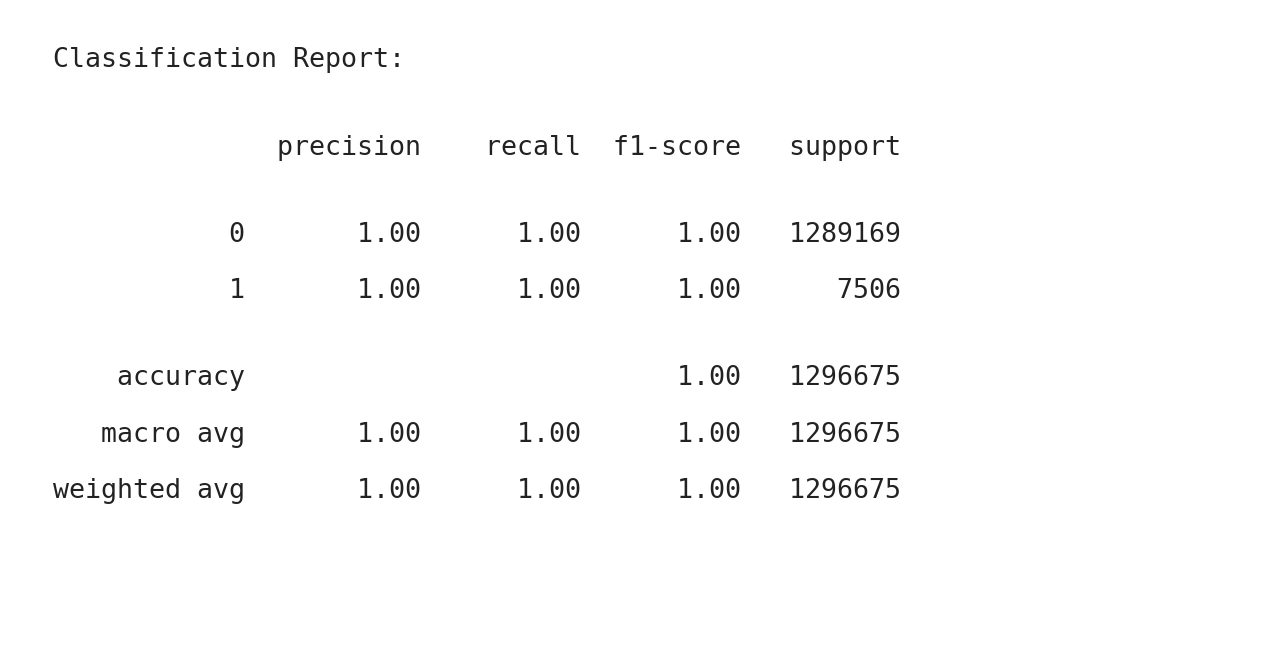
\includegraphics[width=\linewidth,height=0.48\textheight,keepaspectratio]{demo_classification_report.png}

    \column{0.49\textwidth}
    \centering
    {\small Confusion Matrix}\\[0.1cm]
    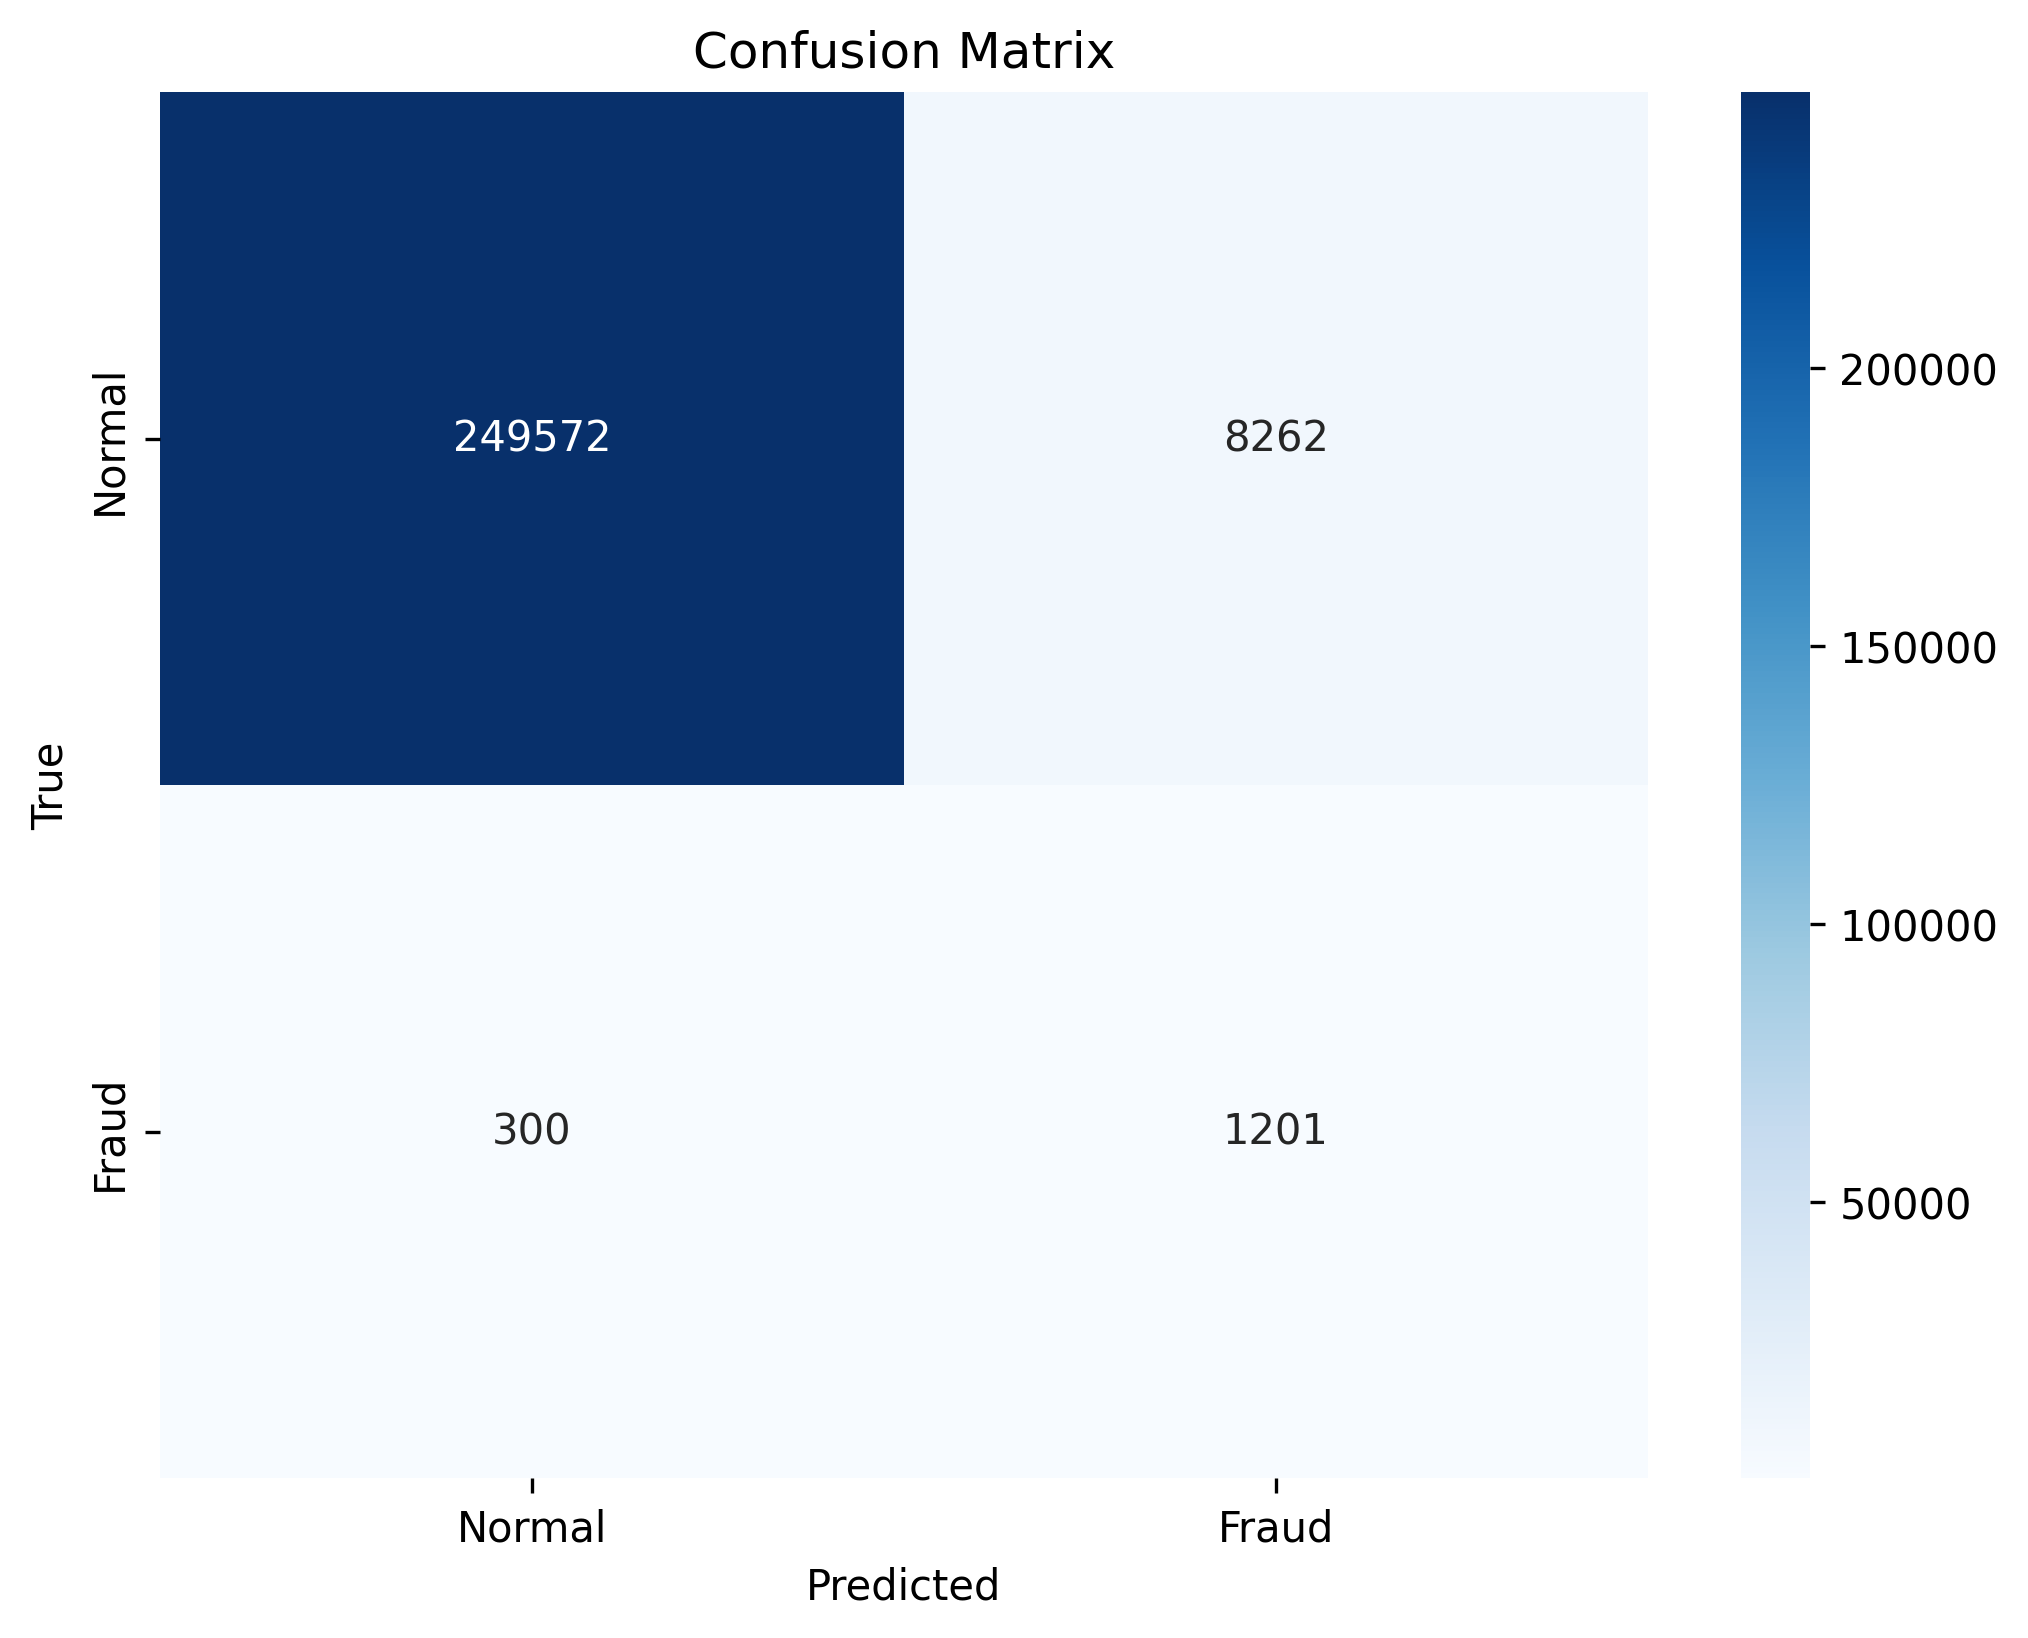
\includegraphics[width=\linewidth,height=0.48\textheight,keepaspectratio]{demo_confusion_matrix.png}
\end{columns}
\end{frame}

\begin{frame}{General Conclusion}
\begin{itemize}
    \item The dataset is imbalanced; in future work we plan to handle this with methods such as SMOTE and other imbalance-aware models.
    \item Some weak-impact features will be tested further and may be removed in future iterations.
    \item Strong signals include: transaction amount (\texttt{amt}), hour (especially late-night), category, and merchant.
    \item Combining weaker features can still create stronger engineered features and improve prediction power.
\end{itemize}
\end{frame}

\begin{frame}{Recommended Next Steps}
\begin{itemize}
    \item Feature engineering: amount transforms, time features, categorical encodings.
    \item Modeling with class imbalance handling:
    \begin{itemize}
        \item class weights, focal loss, or resampling
    \end{itemize}
    \item Evaluate with fraud-focused metrics: PR-AUC, recall, precision.
\end{itemize}
\end{frame}

\begin{frame}
    \centering
    \Huge Thank you
\end{frame}

\end{document}
